\documentclass[11pt, twoside, a4paper]{article}
\usepackage[italian]{babel}
\usepackage[utf8]{inputenc}
\usepackage{amsmath}
\usepackage[cm]{fullpage}
\usepackage{graphicx}
\usepackage{booktabs}
\usepackage{wrapfig}
\usepackage{multirow}
\usepackage{sidecap}
\usepackage{siunitx}
\usepackage{array}
\usepackage[font=small]{caption}
\usepackage[bookmarks, hidelinks]{hyperref}
\usepackage{float}
\usepackage{wrapfig}
\usepackage{titlesec}
\usepackage{subcaption}

\titlespacing\section{0pt}{10pt plus 4pt minus 4pt}{8pt plus 2pt minus 4pt}
\titlespacing\subsection{0pt}{10pt plus 4pt minus 4pt}{8pt plus 2pt minus 4pt}
\titlespacing\subsubsection{0pt}{10pt plus 4pt minus 4pt}{8pt plus 2pt minus 4pt}

\begin{document}

\begin{center}

        {\huge Titolo relazione}
    \vspace{0.1cm}

      	{Francesco Pasa, Andrea Miani - Gruppo B11} \\
      	{francescopasa@gmail.com - 24 febbraio 2014}
    \vspace{-0.2cm}

\end{center}

\section*{Obbiettivo}

\section*{Circuito}

\section*{Dati e risultati}

\subsection{Diodo 1N4007}

Per studiare la caratteristica $I-V$ (corrente-tensione) di un diodo 1N4007 sia in polarizzazione inversa che in diretta ci siamo mossi come segue: abbiamo collegato il diodo all'alimentatore di tensione continua e abbiamo misurato con il multimetro la corrente passante per il diodo.
Ricordiamo che durante questa prima fase dell'esperienza abbiamo prestato attenzione che la corrente attraversante il diodo non superasse i $700\,\si{\milli\ampere}$.
Grazie ai dati misurati abbiamo graficato la curva caratteristica $I-V$ del diodo, mostrata in Figura \ref{fig:diodo}.

%\begin{SCfigure}[1][b!]
\begin{SCfigure}
    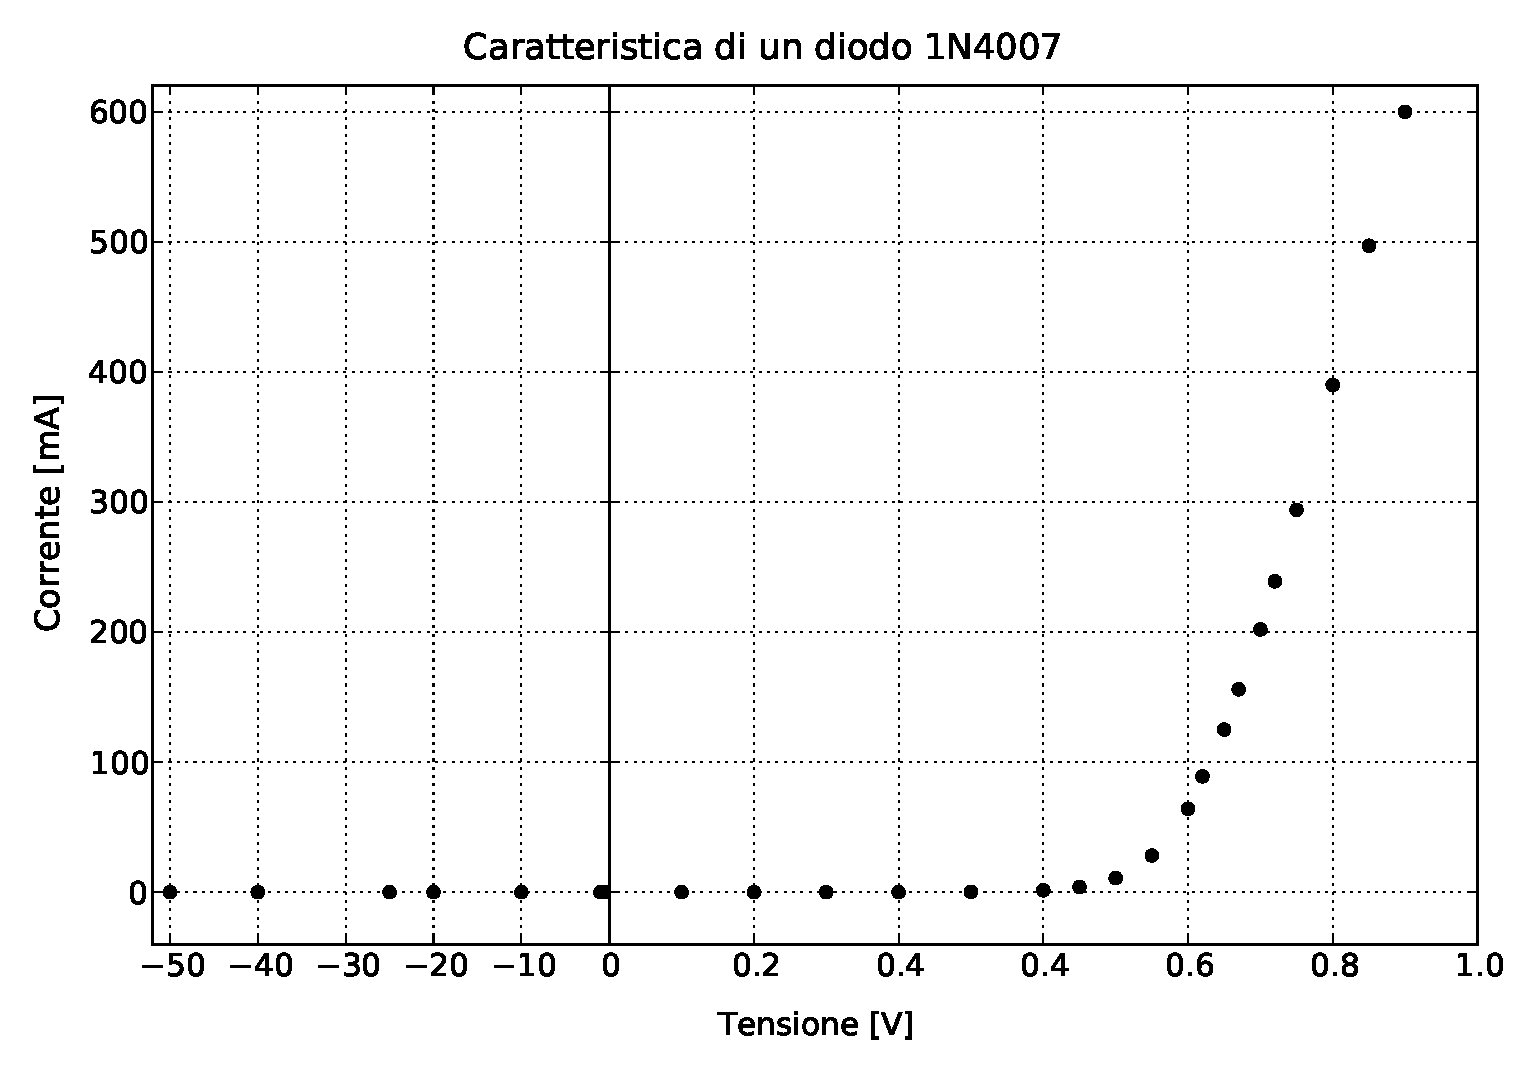
\includegraphics[scale=0.50]{diodo.pdf}
    \caption{La figura mostra la caratteristica corrente-tensione ($I-V$) di un diodo 1N4007. Questo tipo di diodi ha una tensione di breakdown di circa 1000 V, valori che con il nostro alimentatore non siamo in grado di raggiungere.
    La corrente di leakage è praticamente inesistente, mentre la tensione di cut-in è di circa 0.5 V, valore vicino al valore tipico di 0.6 V dei diodi al silicio. }
    \label{fig:diodo}
\end{SCfigure}
%\end{SCfigure}

\subsection{Cella fotovoltaica}

Come secondo obbiettivo abbiamo valutato la caratteristica $I-V$ di una cella fotovoltaica monocristallina al silicio. Questo andamento è stato valutato sia ponendo la cella fotovoltaica al buio, ovvero ponendola all'interno del proprio involucro di cartone, sia esponendola ad una sorgente luminosa.
Come nel caso precedente abbiamo misurato mediante il multimetro la correte passante nella cella fotovoltaica pe poi studiane l'andamento in funzione della tensione.
Anche in questo caso abbiamo dovuto fare attenzione che la corrente massima nella cella fotovoltaica non superasse i $100\,\si{\milli\ampere}$.

\begin{SCfigure}
    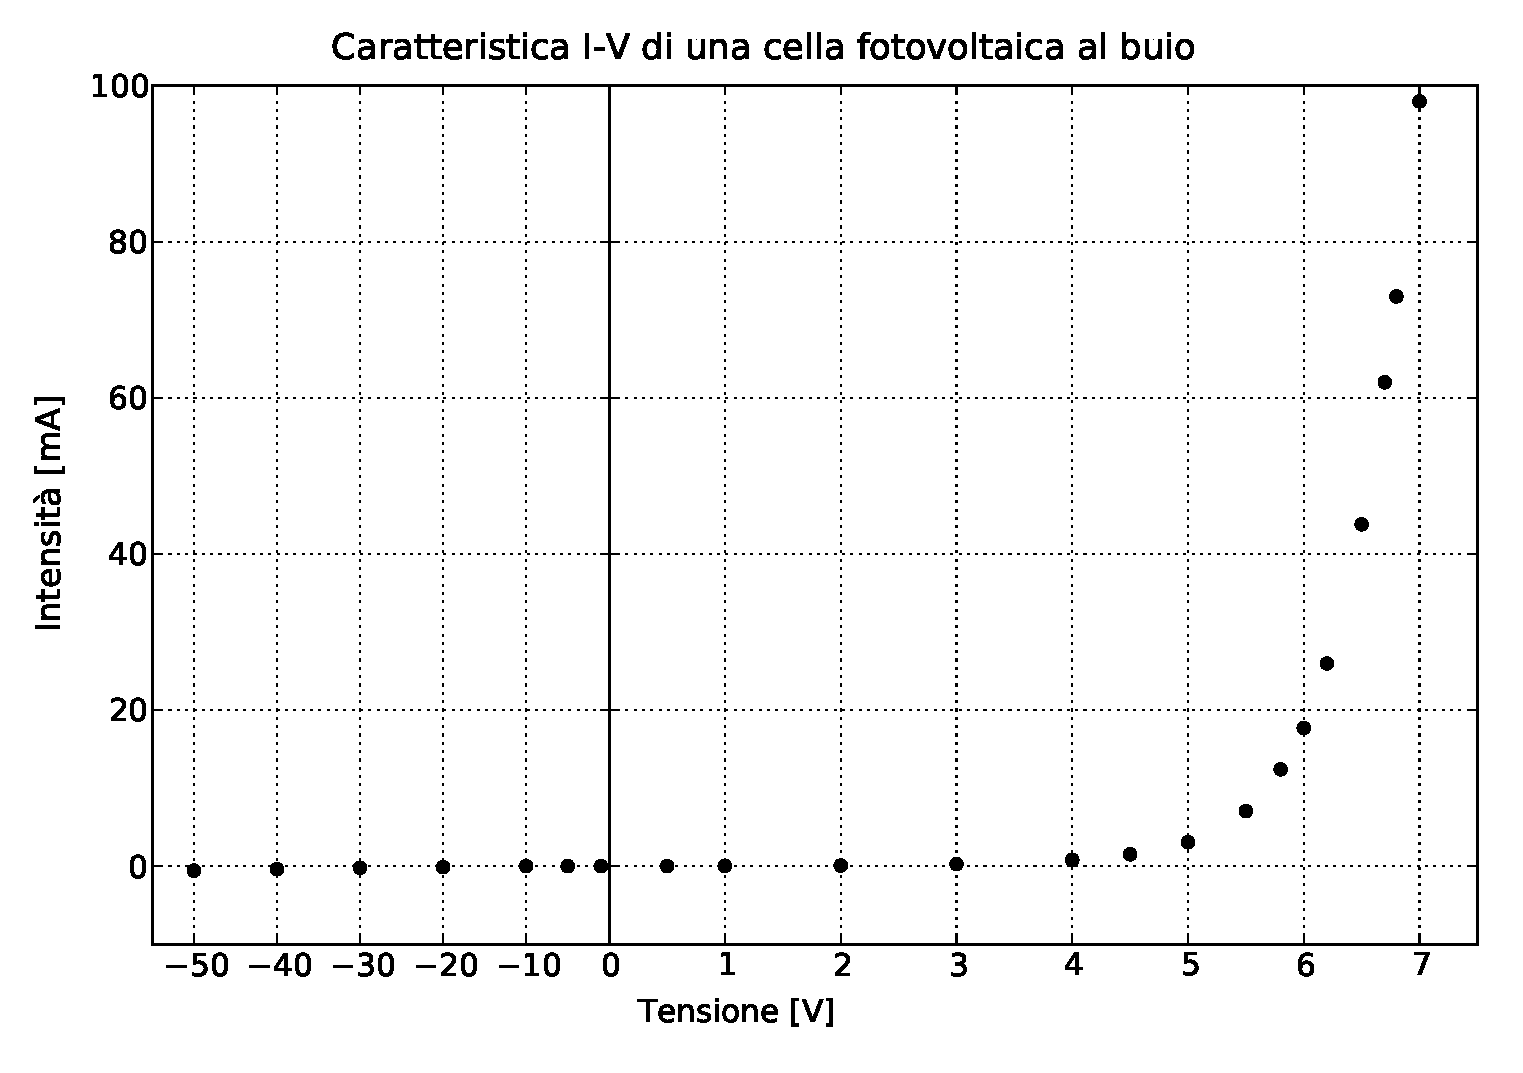
\includegraphics[scale=0.5]{buio.pdf}
    \caption{La caratteristica I-V di una cella fotovoltaica monocristallina al silicio al buio è per molti aspetti simile alla caratteristica di un diodo, con la differenza che la tensione di attivazione è di circa 5 V.}
    \label{fig:buio}
\end{SCfigure}

\begin{SCfigure}
    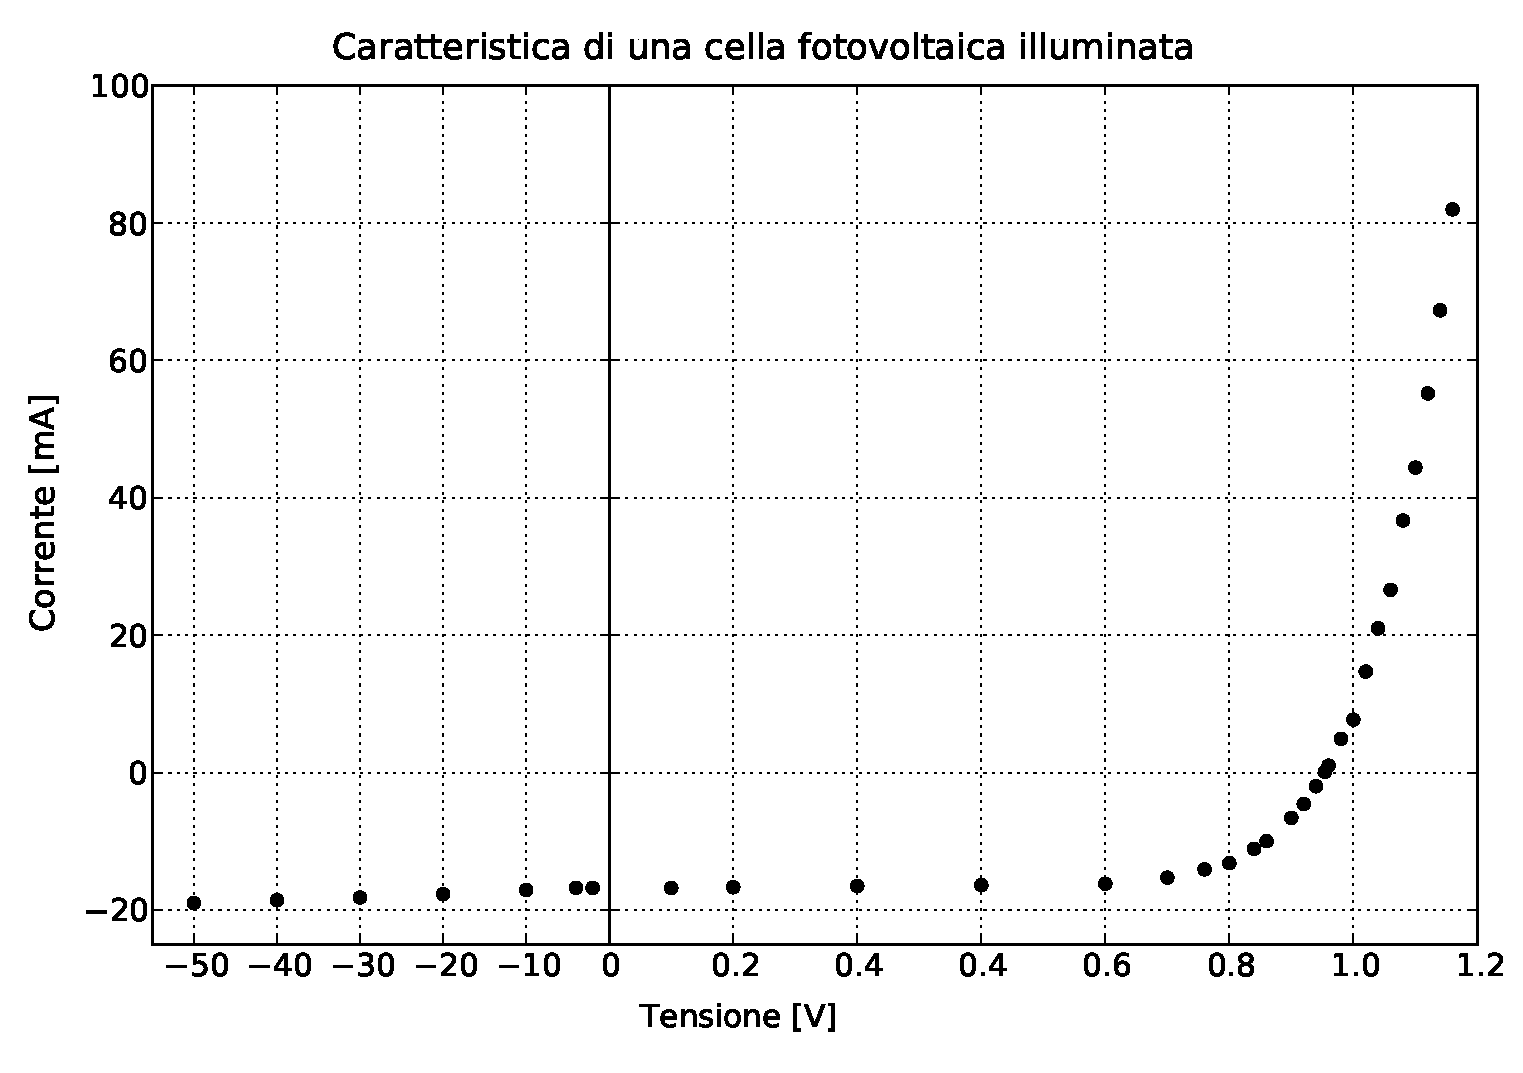
\includegraphics[scale=0.5]{luce.pdf}
    \caption{Questo grafico ilustra la carateristica $I-V$ di una cella fotovoltaica al silicio esposta ad una sorgente luminosa. Sotto queste condizioni, la curva caratteristica varia.}
    \label{fig:luce}
\end{SCfigure}

Infine abbiamo calcolato il FillFactor. Il rapporto tra il prodotto $I_m$ e $V_m$ (rispettivamente i valori di intensità di corrente e tensione il cui rapporto è massimo e quindi la potenza ottenibile dalla cella è massima, ossia in corrispondenza del ginocchio della curva) e il prodotto tra $I\ped{sc}$ e $V\ped{oc}$ (che indicano rispettivamente la corrente di corto circuito per la tensione a vuoto) è chiamato appunto FillFactor o fattore di riempimento della cella.
Il FillFactor dà un’indicazione delle prestazioni della cella.
Quest’ultimo nelle celle al silicio cristallino assume valori generalmente intorno a 0,75 e 0,80. Il FillFactor è anche un parametro di giudizio sul rendimento della cella: elevati valori di questi parametri sono anche indicatori di migliori prestazioni.

\begin{equation}
	\text{FillFactor} \,=\, \frac{I_m\,\cdot\,V_m}{I\ped{sc}\,\cdot\,V\ped{oc}} \,=\, ...
\end{equation}

\subsection{Ponte Graetz}

In questa parte ell'esperienza abbiamo realizzato un circuito raddrizzatore a ponte di diodi, o ponte di Graetz. Il circuito realizzato è illustrato in Figura \ref{fig:raddrizzatore}, eccetto per la presenza del condensatore, che in questa prima analisi non è utilizzato.
Per realizzare il ponte di Graetz abbiamo utilizzato quattro diodi 1N4007 e un carico resistivo da $10\,\si{\kilo\ohm}$. Di questo circuito ne andremo a gaficare la forma d'onda risultante e ne misureremo l'ampiezza.
Quello che ci aspettiamo di vedere è un segnale che è la somma di una semionda positiva e di una semionda negtiva capovolta (doppia semionda).
Infatti questa soluzione, molto usata negli alimentatori, rende molto più semplice il successivo filtraggio e livellamento della tensione fino ad ottenere una corrente continua, non richiedendo peraltro un trasformatore con doppio avvolgimento a presa centrale.
La forma d'onda che abbiamo ottenuto è la seguente:

\begin{SCfigure}
    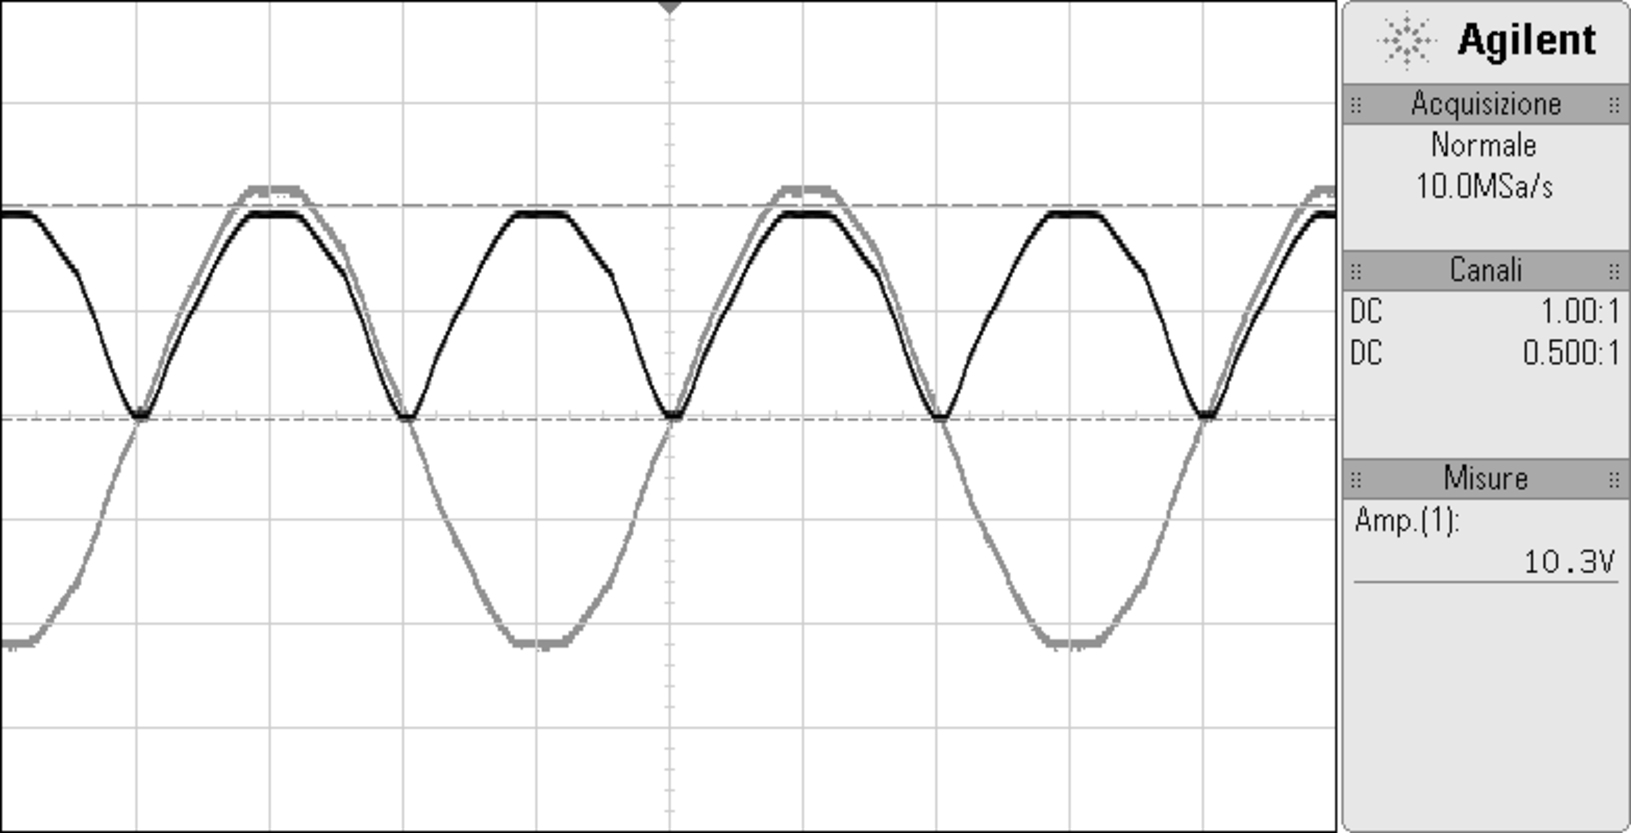
\includegraphics[scale=0.5]{n2_bianco.pdf}
    \caption{L'immagine, direttamente acquisita dall'osciloscopio, mostra con la lina grigia il segnale in ingresso nel nostro circuito (Figura \ref{fig:raddrizzatore}), mentre la linea nera mostra la forma d'onda in uscita dal nostrocircuito. Come ci si aspettava il seganle negativo viene raddrizzato grazie al ponte di diodi. Si può inoltre notare come l'intensità della tensione sia rimasto lo stesso, dal momento che il ponte viene utilizzato solamente come raddrizzatore di corrente.}
    \label{fig:graetz2}
\end{SCfigure}

Successivamente abbiamo studiato la forma d'onda risultante nel caso in cui si variasse la capacità ($C$) del condensatore. Abiamo misurato la frequenza e l'ampiezza del ripple per quattro valori di capacità. Inoltre sempre per glistessi valori abbiamo misurato la tensione $V\ped{m}$ e abbiamo determinato il fattore di ripple.

\begin{equation}
	\text{Fattore di ripple} \,=\, \frac{V\ped{r}}{V\ped{m}}
\end{equation}

dove con $V\ped{r}$ si indica il valore efficace del ripple, ossia dell’ondulazione residua in uscita, mentre con $V\ped{m}$ il valore medio di tensione.
Ricordiamo che il fattore di ripple è la grandezza che caratterizza la qualità di un alimentatore.
I risultati che bbiamo ottenuto sono i seguenti:

%\begin{SCfigure}
\begin{table}[H]
    \centering
    \small
    \begin{tabular}{l c c c}
        \toprule
		Capacità $[\si{\micro\farad}]$ & $V\ped{r} \; [\si{\volt}]$ & $V\ped{m} \, [\si{\volt}]$ & Fattore di ripple \\
        \midrule
		$ 0.500 \pm 0.005 $ & $6.8 \pm 0.1 $ & $ 6.898 \pm 0.001 $ & $ 0.99 \pm 0.01 $ \\
		$ 1.00 \pm 0.01 $ & $ 4.8 \pm 0.1$ & $ 7.73 \pm 0.01 $ & $ 0.62 \pm 0.01$ \\
		$ 2.00 \pm 0.02 $ & $ 3.2 \pm 0.1$ & $ 8.47 \pm 0.01 $ & $ 0.38 \pm 0.01$ \\
		$ 3.00 \pm 0.03 $ & $ 2.4 \pm 0.1$ & $ 8.78 \pm 0.01 $ & $ 0.27 \pm 0.01$ \\
		$ 5.00 \pm 0.05 $ & $ 1.6 \pm 0.1$ & $ 9.07 \pm 0.01 $ & $ 0.18 \pm 0.01$ \\
        \bottomrule
    \end{tabular}
    \caption{In questa tabella sono riportati i valori della tensione media ($V\ped{m}$), della tensione di ripple ($V\ped{r}$) e del fattore di ripple al variare della capacità. La frequenza del segnale in ingresso stata costante per tutte le misure effettuate ed ha valore di $100\,\si{\hertz}$. }
    \label{tab:ripple}
\end{table}
%\end{SCfigure}

%\subsection{Raddrizzatore di tensione a doppia semionda}

%Sfruttando il circuito illustrato in Figura \ref{fig:doppio} abbiamo rietuto l'analisi fatta nel punto precedente è i risultati da noi ottenuti sono i seguenti:

%Capacità	500 nF	1 uF	2 uF	5 uF	3 uF
%Ampiezza picco-picco	6.8 V	4.8 V	3.2 V	1.6 V	2.4 V
%Freq (Hz)	100 Hz	100 Hz	100 Hz	100 Hz	100 Hz
%Media	6.898 V	7.73 V	8.47 V	9.07 V	8.78 V

%[ 0.98579298  0.62095731  0.37780401  0.27334852  0.17640573]

%[ 0.01449766  0.01296153  0.0118148   0.01139378  0.01102707]




\section*{Conclusione}

Pertanto per concludere possiamo osservare che il valore sperimentale di corrente di attivazione dell'interruttore differenziale ($I\ped{exp}$) è compatibile entro la sua inceretezza con quello teorico ($I\ped{teo}$).
Inoltre per quanto riguarda il tempo di intervento, il nostro interruttore ha dimostrato di essere conforme alle norme vigenti, che 
richiedono che tale tempo sia inferiore a 20 ms.


\end{document}
